\documentclass{article}
\usepackage{tikz}
\usetikzlibrary{arrows.meta}
\usepackage{graphicx}
\usepackage{listings}
\usepackage{xcolor}

\definecolor{codegreen}{rgb}{0,0.6,0}
\definecolor{codegray}{rgb}{0.5,0.5,0.5}
\definecolor{codepurple}{rgb}{0.58,0,0.82}
\definecolor{backcolour}{rgb}{0.95,0.95,0.92}

\lstdefinestyle{json}{
    backgroundcolor=\color{backcolour},
    commentstyle=\color{codegreen},
    keywordstyle=\color{magenta},
    numberstyle=\tiny\color{codegray},
    stringstyle=\color{codepurple},
    basicstyle=\ttfamily\footnotesize,
    breakatwhitespace=false,
    breaklines=true,
    captionpos=b,
    keepspaces=true,
    numbers=left,
    numbersep=5pt,
    showspaces=false,
    showstringspaces=false,
    showtabs=false,
    tabsize=2,
    language=json
}

\usepackage{caption}
\usepackage{float}

\title{Analysis Report}
\author{Your Name}
\date{\today}

\begin{document}

\maketitle

\section{Introduction}
This report presents the analysis of various strategies using EPLE results and visual representations through TikZ diagrams.

\section{TikZ Figures}

\begin{figure}[H]
    \centering
    \caption{Addition Diagram}
    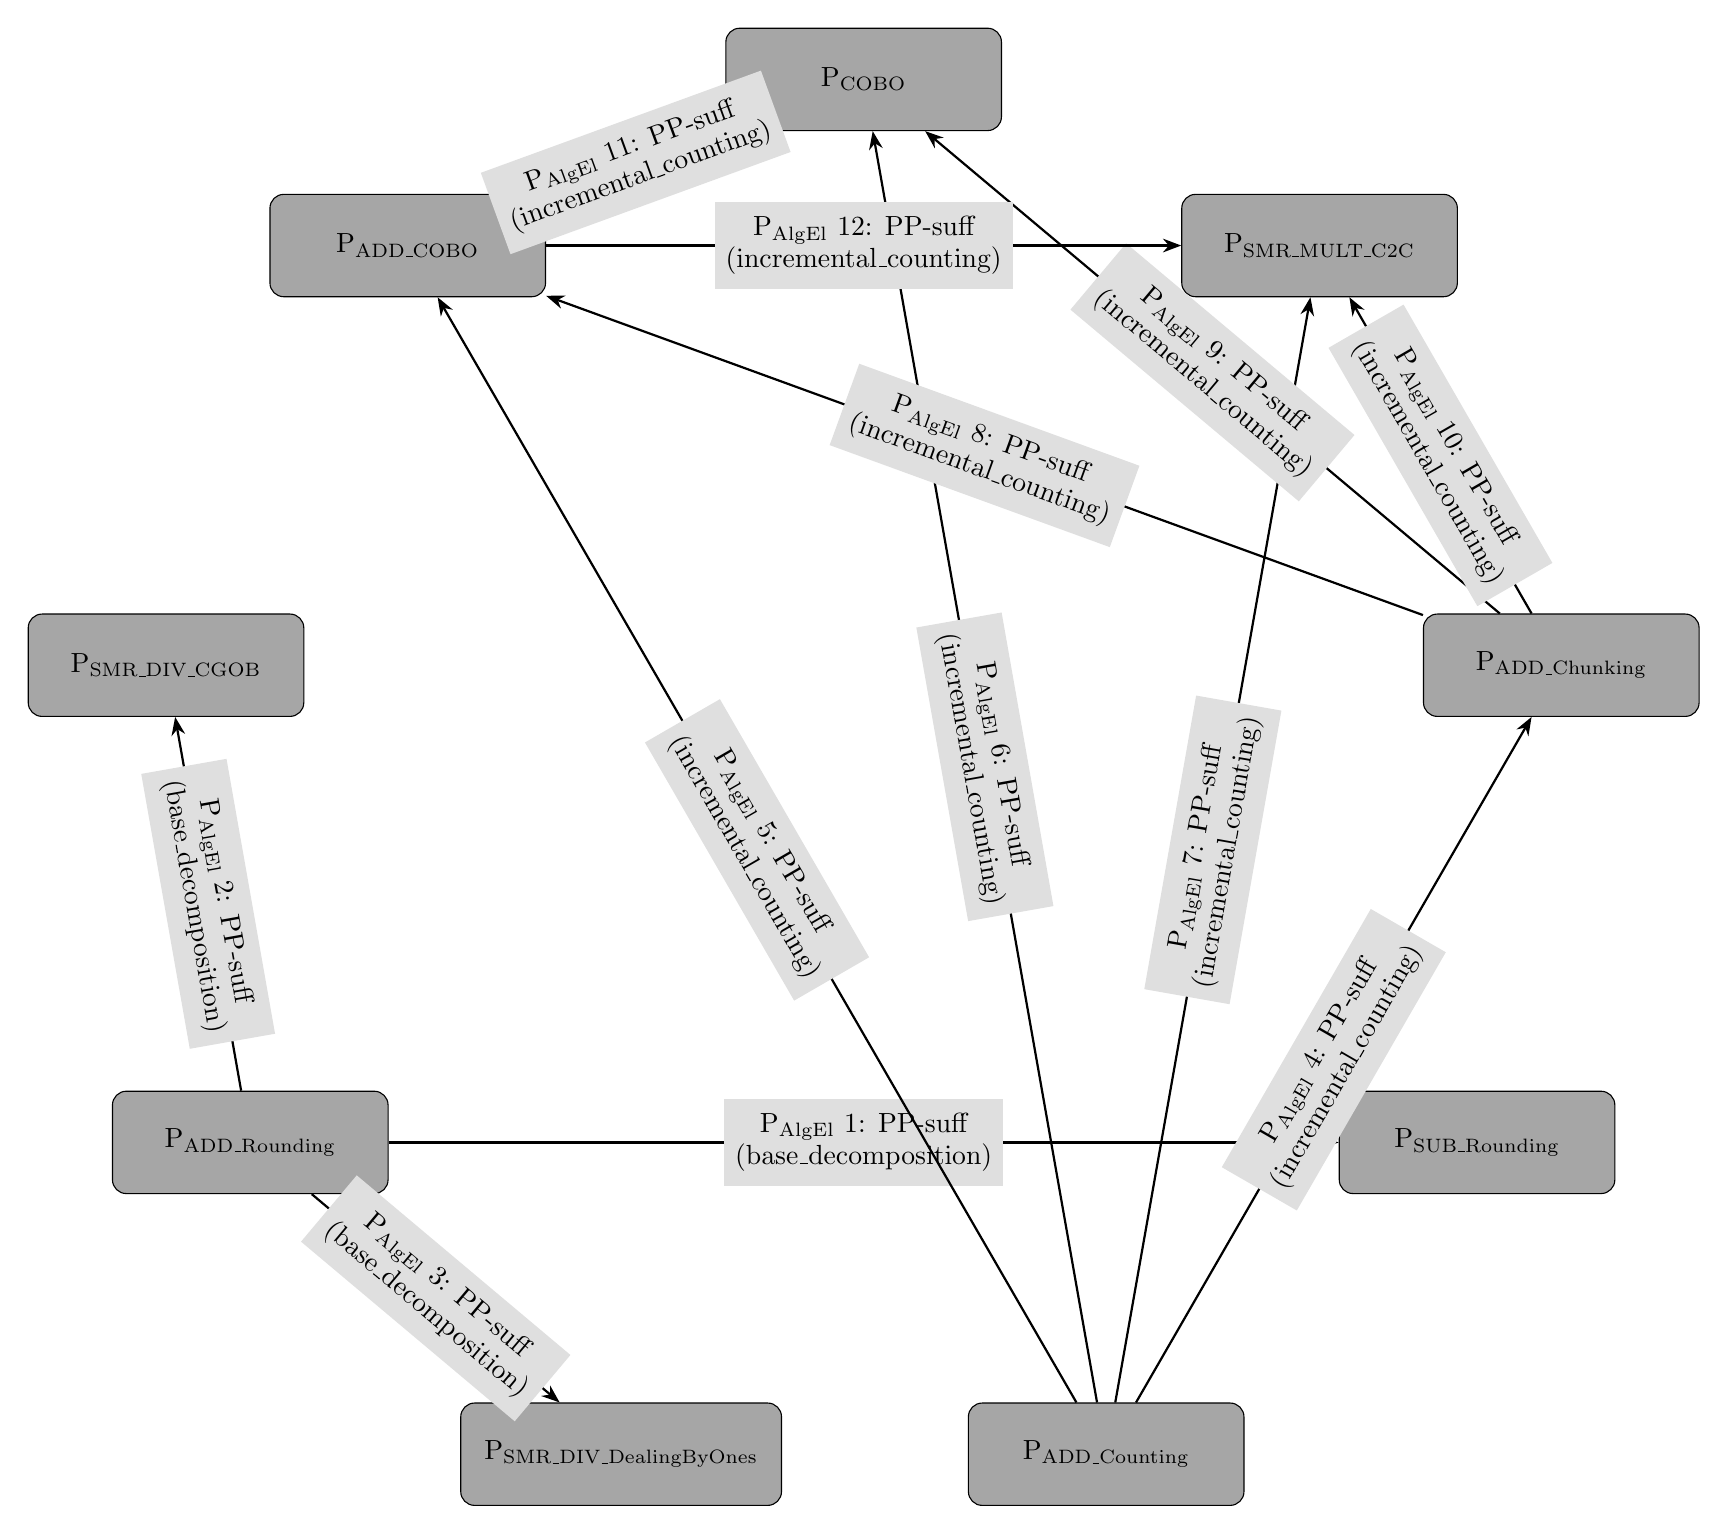
\begin{tikzpicture}[
  % Node Styles
  vnode/.style={ellipse, draw, fill=lightgray!50, text=black, minimum height=1.3cm, minimum width=2.8cm, align=center},
  pnode/.style={rectangle, rounded corners=5pt, draw, fill=gray!70, text=black, minimum height=1.3cm, minimum width=3.5cm, align=center, inner xsep=0.3cm, inner ysep=0.2cm},
  graybox/.style={rectangle, fill=lightgray!50, inner sep=4pt, minimum height=1.1cm, anchor=center, align=center, text centered},
  % Arrow Styles
  solidarrow/.style={-Stealth, thick},
  dashedarrow/.style={dashed, -Stealth, thick, gray},
  textarrow/.style={align=center, inner sep=1pt}
]
\tikzset{font=\linespread{0.8}\selectfont}

% Diagram for: addition

\node[pnode] (P_0) at (0.00,9.00) {P\textsubscript{COBO}};
\node[pnode] (P_1) at (5.79,6.89) {P\textsubscript{SMR\_MULT\_C2C}};
\node[pnode] (P_2) at (8.86,1.56) {P\textsubscript{ADD\_Chunking}};
\node[pnode] (P_3) at (7.79,-4.50) {P\textsubscript{SUB\_Rounding}};
\node[pnode] (P_4) at (3.08,-8.46) {P\textsubscript{ADD\_Counting}};
\node[pnode] (P_5) at (-3.08,-8.46) {P\textsubscript{SMR\_DIV\_DealingByOnes}};
\node[pnode] (P_6) at (-7.79,-4.50) {P\textsubscript{ADD\_Rounding}};
\node[pnode] (P_7) at (-8.86,1.56) {P\textsubscript{SMR\_DIV\_CGOB}};
\node[pnode] (P_8) at (-5.79,6.89) {P\textsubscript{ADD\_COBO}};

\draw[solidarrow] (P_6) -- node[graybox, midway, sloped] {P\textsubscript{AlgEl} 1: PP-suff \\ (base\_decomposition)} (P_3);
\draw[solidarrow] (P_6) -- node[graybox, midway, sloped] {P\textsubscript{AlgEl} 2: PP-suff \\ (base\_decomposition)} (P_7);
\draw[solidarrow] (P_6) -- node[graybox, midway, sloped] {P\textsubscript{AlgEl} 3: PP-suff \\ (base\_decomposition)} (P_5);
\draw[solidarrow] (P_4) -- node[graybox, midway, sloped] {P\textsubscript{AlgEl} 4: PP-suff \\ (incremental\_counting)} (P_2);
\draw[solidarrow] (P_4) -- node[graybox, midway, sloped] {P\textsubscript{AlgEl} 5: PP-suff \\ (incremental\_counting)} (P_8);
\draw[solidarrow] (P_4) -- node[graybox, midway, sloped] {P\textsubscript{AlgEl} 6: PP-suff \\ (incremental\_counting)} (P_0);
\draw[solidarrow] (P_4) -- node[graybox, midway, sloped] {P\textsubscript{AlgEl} 7: PP-suff \\ (incremental\_counting)} (P_1);
\draw[solidarrow] (P_2) -- node[graybox, midway, sloped] {P\textsubscript{AlgEl} 8: PP-suff \\ (incremental\_counting)} (P_8);
\draw[solidarrow] (P_2) -- node[graybox, midway, sloped] {P\textsubscript{AlgEl} 9: PP-suff \\ (incremental\_counting)} (P_0);
\draw[solidarrow] (P_2) -- node[graybox, midway, sloped] {P\textsubscript{AlgEl} 10: PP-suff \\ (incremental\_counting)} (P_1);
\draw[solidarrow] (P_8) -- node[graybox, midway, sloped] {P\textsubscript{AlgEl} 11: PP-suff \\ (incremental\_counting)} (P_0);
\draw[solidarrow] (P_8) -- node[graybox, midway, sloped] {P\textsubscript{AlgEl} 12: PP-suff \\ (incremental\_counting)} (P_1);

\end{tikzpicture}
    \label{fig:add}
\end{figure}

\begin{figure}[H]
    \centering
    \caption{Miscellaneous Diagram}
    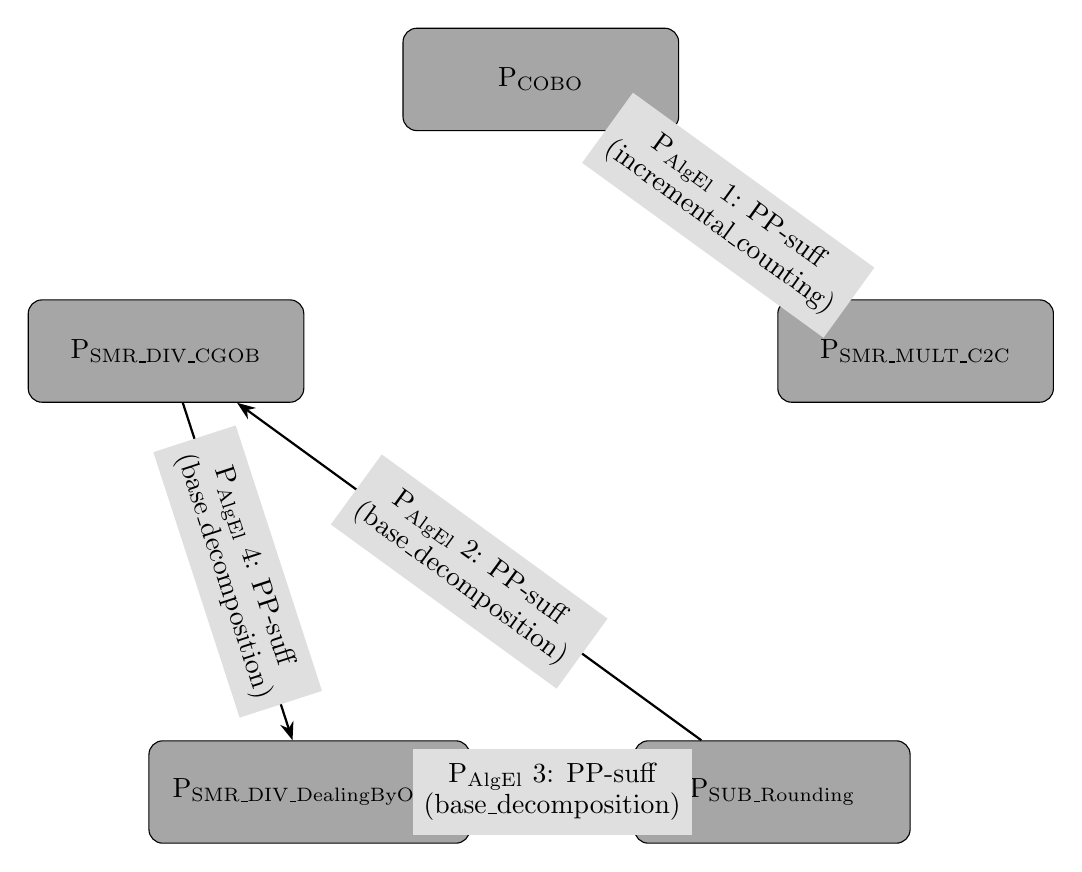
\begin{tikzpicture}[
  % Node Styles
  vnode/.style={ellipse, draw, fill=lightgray!50, text=black, minimum height=1.3cm, minimum width=2.8cm, align=center},
  pnode/.style={rectangle, rounded corners=5pt, draw, fill=gray!70, text=black, minimum height=1.3cm, minimum width=3.5cm, align=center, inner xsep=0.3cm, inner ysep=0.2cm},
  graybox/.style={rectangle, fill=lightgray!50, inner sep=4pt, minimum height=1.1cm, anchor=center, align=center, text centered},
  % Arrow Styles
  solidarrow/.style={-Stealth, thick},
  dashedarrow/.style={dashed, -Stealth, thick, gray},
  textarrow/.style={align=center, inner sep=1pt}
]
\tikzset{font=\linespread{0.8}\selectfont}

% Diagram for: miscellaneous

\node[pnode] (P_0) at (0.00,5.00) {P\textsubscript{COBO}};
\node[pnode] (P_1) at (4.76,1.55) {P\textsubscript{SMR\_MULT\_C2C}};
\node[pnode] (P_2) at (2.94,-4.05) {P\textsubscript{SUB\_Rounding}};
\node[pnode] (P_3) at (-2.94,-4.05) {P\textsubscript{SMR\_DIV\_DealingByOnes}};
\node[pnode] (P_4) at (-4.76,1.55) {P\textsubscript{SMR\_DIV\_CGOB}};

\draw[solidarrow] (P_0) -- node[graybox, midway, sloped] {P\textsubscript{AlgEl} 1: PP-suff \\ (incremental\_counting)} (P_1);
\draw[solidarrow] (P_2) -- node[graybox, midway, sloped] {P\textsubscript{AlgEl} 2: PP-suff \\ (base\_decomposition)} (P_4);
\draw[solidarrow] (P_2) -- node[graybox, midway, sloped] {P\textsubscript{AlgEl} 3: PP-suff \\ (base\_decomposition)} (P_3);
\draw[solidarrow] (P_4) -- node[graybox, midway, sloped] {P\textsubscript{AlgEl} 4: PP-suff \\ (base\_decomposition)} (P_3);

\end{tikzpicture}
    \label{fig:misc}
\end{figure}
\section{EPLE Results}
\lstinputlisting[style=json]{data/eple_results.json}

\section{Analysis Results}
\lstinputlisting[style=json]{data/analysis_results.json}


\section{Conclusion}
This report summarizes the findings from the analysis and visualizations provided.

\end{document}